\documentclass[conference]{IEEEtran}
\IEEEoverridecommandlockouts

\usepackage{cite}
\usepackage{amsmath,amssymb,amsfonts}
\usepackage{amsthm}
\usepackage{graphicx}
\usepackage{textcomp}
\usepackage{xcolor}
\usepackage{booktabs}
\usepackage{microtype}
\usepackage{algorithm}
\usepackage{algorithmic}
\usepackage{tikz}
\usetikzlibrary{arrows.meta,positioning,fit,backgrounds,shapes.geometric}
\usepackage[hidelinks]{hyperref}
\usepackage{balance}

\newtheorem{lemma}{Lemma}

\def\BibTeX{{\rm B\kern-.05em{\sc i\kern-.025em b}\kern-.08em
T\kern-.1667em\lower.7ex\hbox{E}\kern-.125emX}}

% Small helper
\newcommand{\todo}[1]{\textcolor{red}{[TODO: #1]}}

\begin{document}

% ------------------------------------------------------------
\title{Pixel Block Chain: Spatial Tamper Localization and Crop-Resilient Edit Ledger for Images in the Wild}

\author{
  \IEEEauthorblockN{Fran\c{c}ois L\'{e}gare}
  \IEEEauthorblockA{Independent Researcher\\
    Montr\'{e}al, Qu\'{e}bec, Canada\\
    flegare@gmail.com}
  \and
  \IEEEauthorblockN{Sion Israel Sion}
  \IEEEauthorblockA{\textit{Department of Software and IT Engineering}\\
    \textit{\'{E}cole de technologie sup\'{e}rieure}\\
    Montr\'{e}al, QC, Canada\\
    sion-israel.sion.1@ens.etsmtl.ca}
  \and
  \IEEEauthorblockN{Alain April}
  \IEEEauthorblockA{\textit{Department of Software and IT Engineering}\\
    \textit{\'{E}cole de technologie sup\'{e}rieure}\\
    Montr\'{e}al, QC, Canada\\
    alain.april@etsmtl.ca}
}


\maketitle
% --- Camera-ready copyright notice: replace ISBN with the exact ICIP 2026 string ---

\IEEEpubid{\makebox[\columnwidth]{XXX-X-XXXX-XXXX-X/26/\$31.00~\copyright2026~IEEE\hfill}\hspace{\columnsep}\makebox[\columnwidth]{}}

% ------------------------------------------------------------
\begin{abstract}
Images shared through social media, messaging platforms, and editorial workflows routinely lose their external provenance manifests through transcoding, cropping, and metadata stripping. Manifest-based systems such as C2PA address provenance at the file-container level, and recent durable-credential mechanisms add rediscovery paths, but neither provides a self-contained, tile-local integrity ledger when only pixels remain. This paper presents Pixel Block Chain (PBC), a lightweight, learning-free watermarking scheme that embeds a grid of independent hash-linked chains directly into image least-significant bits. PBC targets lossless and near-lossless distribution channels (archival masters, editorial handoffs, and wire-service exchanges) rather than lossy social-media re-encoding, and it provides tile-local integrity rather than cryptographic identity. The scheme enables spatial tamper localization and partial Edit Ledger recovery after redistribution within this regime. Each image tile carries its own chain, and a break in one tile does not cascade to adjacent regions, a property we prove formally. A compliant editor can append records only to modified tiles, preserving an auditable, region-level Edit Ledger.
For crop-heavy distribution paths, PBC-Forest plants independent genesis blocks at pseudo-random positions, achieving 41.1 to 44.6\% fragment survival after severe non-aligned cropping where the regular-grid baseline collapses to 0\%. On a 99-image benchmark spanning real photographs and synthetic content, PBC achieves a mean PSNR of $51.2$\,dB at embedding depth $k{=}1$, and, under a synthetic rectangular tampering protocol, 100\% tile-level tamper detection with 0\% false positives, using no neural encoder and no external service dependency.
\end{abstract}


\begin{IEEEkeywords}
image forensics, tamper localization, fragile watermarking, edit ledger, steganography, crop resilience, multimedia security
\end{IEEEkeywords}

% ============================================================
\section{Introduction}
\label{sec:intro}

\IEEEpubidadjcol
The integrity of digital images is increasingly undermined not by
sophisticated forgeries alone, but by the ordinary mechanics of
distribution. A photograph posted to a social platform is transcoded.
A crop is re-shared in a chat thread. A wire-service JPEG is
re-exported through an editing tool. Each step can silently discard
the external metadata that signed provenance systems rely on.

Manifest-based standards such as C2PA~\cite{c2pa_spec} provide a
rigorous chain of identity and claim assertions when the file container
survives end-to-end. Recent durable-credential mechanisms add
rediscovery paths through soft bindings and repositories. The
complementary failure mode we target is equally common: the container
disappears, and with it the local manifest, leaving only the pixel
array and no tile-level tamper signal embedded in the content itself. We state our scope plainly: PBC operates within lossless or near-lossless channels, providing tile-local integrity and edit-ledger continuity rather than robustness to lossy re-encoding or cryptographic authentication of the originator.

Classical fragile watermarking~\cite{he2008blockchain,fang2020blockchain}
embeds integrity signals into pixels, but single-chain architectures
suffer from a cascade property in which one tampered block invalidates
all subsequent blocks, making region-level localization unreliable.
Neural watermarking approaches~\cite{editguard,omniguard} offer
pixel-level localization but require tens of millions of parameters,
placing them out of reach for firmware or lightweight publisher
toolchains.

This paper addresses this gap with Pixel Block Chain (PBC), a
deterministic, learning-free scheme with four contributions:

\begin{enumerate}
  \item A grid-of-chains architecture with a formal cascade-isolation
    property (Lemma~\ref{lem:isolation}), ensuring that spatial
    localization remains reliable even under partial tampering.

  \item A per-tile Edit Ledger with append mode, where compliant
    editors write only to modified tiles, preserving unbroken history
    elsewhere and yielding 13.5 to 74.2\% wall-clock speedups in
    measured append-depth scenarios.

  \item PBC-Forest, a scatter mode achieving 41.1 to 44.6\%
    Edit Ledger fragment survival after severe non-aligned cropping
    where the regular grid offers zero survival.

  \item An open reference implementation validated on 99 images with
    $51.2$\,dB mean PSNR and, under a synthetic tampering protocol, 100\% tile-level detection with
    0\% false positives.
\end{enumerate}

% ============================================================
\section{Related Work}
\label{sec:related}

\subsection{Fragile Watermarking and Tamper Localization}

Fragile watermarking for tamper localization has been studied for over
two decades~\cite{cox2007watermarking}. He~et~al.~\cite{he2008blockchain}
introduced a block-chain structure for per-block integrity, but their
scheme links all blocks into a single global chain. Modifying any block
therefore invalidates all downstream blocks, preventing reliable spatial
localization of the actual tampered region.
Fang~et~al.~\cite{fang2020blockchain} extend this idea to a
blockchain-backed restoration scheme that inherits the same cascade
fragility. In a broader survey of the field,
Korus~\cite{korus2017survey} identifies cascade propagation as the
central barrier to practical spatial forensics.

Semi-fragile schemes~\cite{lin2001semifragile} take a different approach
by tolerating benign processing such as JPEG compression and mild
resizing. This tolerance comes at the cost of localization precision,
because the margin that absorbs legitimate processing also masks
deliberate small-region edits. PBC targets the complementary regime of
lossless or near-lossless channels where full sensitivity is desirable
and where the distinction between benign and malicious modification need
not be approximated.

\subsection{Neural Watermarking}

Where classical schemes embed hand-crafted signals, neural watermarking
relies on learned representations.
EditGuard~\cite{editguard} and OmniGuard~\cite{omniguard} use trained
encoder-decoder networks to embed provenance and achieve pixel-level
localization with some robustness to lossy compression. However, their
inference pipelines require tens of millions of parameters and GPU-class
hardware, precluding deployment in camera firmware, air-gapped archival
workflows, or lightweight publisher scripts. On the image quality axis, LSB embedding at $k{=}1$ yields $51.2$\,dB, above the values typically reported for EditGuard (${\sim}40$\,dB) and OmniGuard (${\sim}38$\,dB). We read this gap as a consequence of divergent design points rather than a like-for-like advantage: neural schemes deliberately trade fidelity for survival across the lossy channels that PBC does not target.

\subsection{Manifest-Based Provenance}

C2PA~\cite{c2pa_spec} and Project Origin~\cite{aythora2020origin}
ground provenance in signed assertions stored in the file container.
C2PA v2.4 further defines durable credentials, fingerprint-based
rediscovery, invisible watermarks, and manifest repositories to improve
resilience after redistribution. These mechanisms strengthen the
container-level provenance chain but do not embed a per-tile integrity
ledger into the pixel array itself. PBC is designed as a complementary
layer that treats the pixel content as the verification substrate,
activated precisely when container-level mechanisms are unavailable.

\subsection{Robustness to Redistribution}

Social-media distribution subjects images to cropping, resampling, and
lossy re-encoding. Prior fragile schemes collapse entirely after
non-aligned cropping because genesis-block positions are destroyed by
the spatial shift~\cite{korus2017survey}. Rather than pursuing
compression robustness, which is the goal of semi-fragile
schemes~\cite{lin2001semifragile}, PBC-Forest takes a statistical
approach. By planting genesis blocks at pseudo-random positions across
the image, it maximizes the probability that at least some anchors
survive spatial excision. This enables partial and spatially bounded
Edit Ledger recovery from a crop that would leave a conventional grid
with no readable signal. The design is informed by the observation that
redistribution channels vary widely in the transformations they
apply~\cite{corvi2023synthetic}, and that even partial fragment survival
can provide useful forensic evidence when no other provenance signal
remains.

% ============================================================
\section{Pixel Block Chain}
\label{sec:method}

\subsection{Threat Model}
\label{sec:threat}

We assume the adversary may read and modify any pixel of the embedded
image, knows the PBC format, and may attempt to write blocks claiming
arbitrary originator identifiers. The adversary is assumed not to know
the encoder's session timestamp $\tau$ at encode time. If $\tau$ is
later disclosed, forgery of a consistent tile chain requires producing
a second preimage of the truncated SHA-256 genesis hash, which we
treat as computationally infeasible at 48-bit truncation for
opportunistic adversaries, though not as a strong cryptographic
guarantee. Accordingly, we position PBC as a tile-local integrity and edit-ledger mechanism rather than a provenance or identity system: it does not authenticate the originator and is not a substitute for signed credentials such as C2PA, with which it is designed to compose rather than compete.

\emph{Goals.} Detect any tile-local pixel modification, localize
modifications to tile granularity, and recover a partial Edit Ledger
when only a non-aligned crop survives.

\emph{Out of scope.} (i) Content-aware modifications that preserve LSB
structure (e.g., careful inpainting onto original-LSB regions);
(ii) cryptographic identity binding, as the originator ID is
self-asserted and not signed; (iii) surviving lossy re-encoding such as
JPEG.

\subsection{Image Partitioning}

PBC partitions a $W \times H$ image into a grid of
$T_x \times T_y$ non-overlapping tiles, where
$T_x = \lceil W / s \rceil$, $T_y = \lceil H / s \rceil$,
and $s = 128$\,px is the default tile side. Edge tiles are zero-padded
to $s \times s$ during embedding and cropped back during extraction.
Each tile $(t_x, t_y)$ is processed independently.

\subsection{Block Format}

Within each tile, PBC embeds a sequence of fixed-size blocks.
At $B = 32$\,bytes each, one block occupies
$\lceil 8B / (3k) \rceil$ pixels at embedding depth $k$.
A tile of $128 \times 128$ pixels at $k{=}1$ holds up to $190$ blocks,
more than sufficient for a full professional post-production session.
Table~\ref{tab:blockformat} details the field layout.

\begin{table}[t]
  \centering
  \caption{PBC block format. Each block occupies 32 bytes.}
  \label{tab:blockformat}
  \begin{tabular}{@{}ll@{}}
    \toprule
    Field & Size \\
    \midrule
    Sync frame                     & 6\,B \\
    Version                        & 1\,B \\
    Originator ID                  & 4\,B \\
    Operation code                 & 2\,B \\
    Block index                    & 2\,B \\
    Tile coordinates $(t_x, t_y)$  & 2\,B \\
    Timestamp delta                & 3\,B \\
    Extension                      & 4\,B \\
    CRC-16                         & 2\,B \\
    Chain hash (truncated SHA-256) & 6\,B \\
    \bottomrule
  \end{tabular}
\end{table}

The \emph{originator ID} is the 32-bit truncated SHA-256 of a
self-asserted identity string, optionally bound to an external
certificate. The \emph{chain hash} is the SHA-256 of the raw bytes of
the immediately preceding block in the same tile. For the genesis block
it is set to a fixed seed $g_0 = \mathrm{SHA256}(\mathit{oid} \,\|\,
t_x \,\|\, t_y \,\|\, \tau)$ truncated to 48 bits,
where $\tau$ is a session timestamp. Blocks are serialized and written
into the $k$ least-significant bits of each RGB channel of the tile
pixels, with $k \in \{1, 2, 3\}$.

\subsection{Architecture Overview}

\begin{figure}[t]
  \centering
  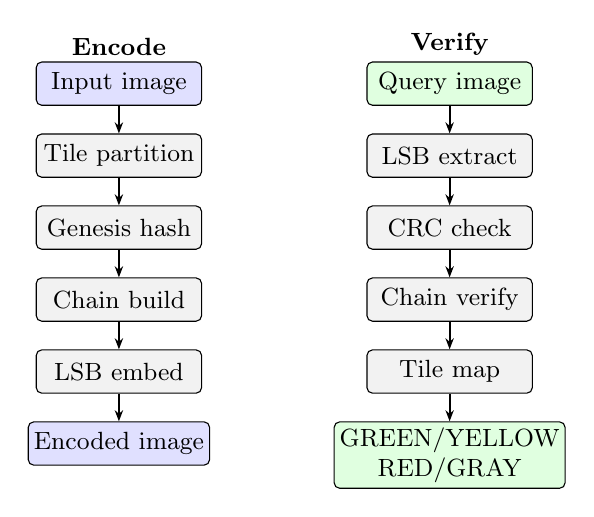
\begin{tikzpicture}[
      font=\small,
      box/.style={draw, rounded corners=2pt, minimum width=2.1cm,
                  minimum height=0.55cm, align=center, fill=gray!10},
      arr/.style={-{Stealth[length=4pt]}, thick},
      every node/.style={inner sep=2pt}
    ]
    % Encode column
    \node[box, fill=blue!12] (img)    at (0,0)    {Input image};
    \node[box] (part)  [below=0.35cm of img]  {Tile partition};
    \node[box] (gen)   [below=0.35cm of part] {Genesis hash};
    \node[box] (chain) [below=0.35cm of gen]  {Chain build};
    \node[box] (lsb)   [below=0.35cm of chain]{LSB embed};
    \node[box, fill=blue!12] (enc)   [below=0.35cm of lsb]  {Encoded image};

    \draw[arr] (img)   -- (part);
    \draw[arr] (part)  -- (gen);
    \draw[arr] (gen)   -- (chain);
    \draw[arr] (chain) -- (lsb);
    \draw[arr] (lsb)   -- (enc);
    \node[above=0pt of img, font=\bfseries\small] {Encode};

    % Verify column
    \node[box, fill=green!12] (vimg)  at (4.2,0)   {Query image};
    \node[box] (ext)   [below=0.35cm of vimg]  {LSB extract};
    \node[box] (crc)   [below=0.35cm of ext]   {CRC check};
    \node[box] (hchk)  [below=0.35cm of crc]   {Chain verify};
    \node[box] (map)   [below=0.35cm of hchk]  {Tile map};
    \node[box, fill=green!12] (out)   [below=0.35cm of map]   {GREEN/YELLOW\\RED/GRAY};

    \draw[arr] (vimg) -- (ext);
    \draw[arr] (ext)  -- (crc);
    \draw[arr] (crc)  -- (hchk);
    \draw[arr] (hchk) -- (map);
    \draw[arr] (map)  -- (out);
    \node[above=0pt of vimg, font=\bfseries\small] {Verify};
  \end{tikzpicture}
  \caption{PBC encode and verify pipelines. Tile independence means any
    tile can be verified in isolation; a failure in one tile does not
    affect adjacent tile outcomes.}
  \label{fig:arch}
\end{figure}

Fig.~\ref{fig:arch} shows the encode and verify pipelines. Verification
produces one of four tile states: GREEN (chain present and internally
consistent), YELLOW (continuity changed by a compliant edit), RED
(chain breaks inconsistently with any known compliant operation), or
GRAY (no PBC data detected).

\subsection{Cascade Isolation by Construction}

PBC's grid-of-chains is designed so that tile chains never reference
each other. We formalize this property below for use in subsequent
claims.

\begin{lemma}[Cascade isolation by construction]
\label{lem:isolation}
In PBC's grid-of-chains architecture, the verification outcome of tile
$(t_x, t_y)$ is independent of the verification outcome of any other
tile $(t_x', t_y')$ with $(t_x', t_y') \neq (t_x, t_y)$.
\end{lemma}

\begin{proof}[Proof sketch]
Each chain hash in tile $(t_x, t_y)$ is computed exclusively over bytes
of the preceding block within that tile. No field in any block
references data from another tile. A modification to tile $(t_x, t_y)$
changes the genesis hash of that tile and all subsequent chain hashes
within it, but leaves every byte of every block in $(t_x', t_y')$
unchanged. Because the verification predicate for $(t_x', t_y')$ is a
function only of the blocks it reads, its outcome is unaffected.
\end{proof}

This contrasts directly with single-chain
schemes~\cite{he2008blockchain,fang2020blockchain}, where one modified
block cascades to invalidate all downstream integrity checks.

\subsection{Per-Tile Edit Ledger and Append Mode}

A \emph{genesis} block is written at encode time. Subsequent
\emph{append} blocks are written by any compliant editor that modifies a
tile. If only subset $S \subseteq \mathcal{T}$ of tiles change, append
mode reads the existing chain in each $t \in S$, appends one new block
carrying the edit metadata and updated chain hash, and writes back only
those tiles. The Edit Ledger answers not only \emph{whether} the image
changed but \emph{where} edit continuity was preserved versus where a
new action occurred. Partial-image append is faster than full re-encode
because the unmodified $|\mathcal{T}| - |S|$ tiles are never touched.

\subsection{PBC-Forest: Crop-Resilient Scatter Mode}

A non-aligned crop shifts the pixel array relative to tile boundaries,
destroying all block synchronization in grid mode. PBC-Forest replaces
the deterministic tile grid with pseudo-random 32-byte genesis block
placement at non-overlapping 86-pixel-aligned slots:

\begin{algorithm}[t]
  \caption{PBC-Forest Encode}
  \label{alg:forest}
  \begin{algorithmic}[1]
    \REQUIRE Image $I$, originator ID $\mathit{oid}$, anchor count $N_f$, seed $q$
    \STATE $m \leftarrow \lfloor WH / 86 \rfloor$
    \STATE $S \leftarrow [0, 86, 172, \ldots, 86(m{-}1)]$
    \STATE $\mathrm{shuffle}(S, \mathrm{PRNG}(q))$
    \STATE $A \leftarrow S[0:\min(N_f,m)]$ \COMMENT{non-overlapping pixel slots}
    \FORALL{$i,p \in A$}
      \STATE $(u,v) \leftarrow (i \bmod 256, \lfloor i/256 \rfloor \bmod 256)$
      \STATE $g_i \leftarrow \mathrm{SHA256}(\mathit{oid}\,\|\,u\,\|\,v\,\|\,\tau)$ truncated to 48 bits
      \STATE Write one genesis block at flat pixel index $p$ with $(t_x,t_y)=(u,v)$
    \ENDFOR
    \RETURN embedded image, seed $q$
  \end{algorithmic}
\end{algorithm}

At verify time the receiver scans the image for sync frames and
CRC-valid blocks, then verifies each block whose genesis hash matches
its embedded forest index. Any anchor whose 86-pixel span survived the
crop is recovered independently.
Forest mode does not survive content-altering lossy compression; it
survives \emph{spatial excision} (cropping, padding, aspect-ratio
change) by statistical coverage: with enough anchors, at least some
positions survive most practically occurring crops.

% ============================================================
\section{Experiments}
\label{sec:experiments}

\subsection{Setup}

\textbf{Dataset.} We evaluate PBC on 99 images: 94 real photographs
drawn from COCO~\cite{coco_dataset}, Oxford Flowers~\cite{flowers_dataset},
Oxford-IIIT Pets~\cite{pets_dataset}, and one demonstration photograph
(diverse subjects, textures, and lighting), plus 5 synthetic classes
(portrait, landscape, document, geometric, noise) used as cross-class
consistency probes.

\textbf{Hardware.} Intel Core i9-12900KF, 64\,GB DDR5, Windows~11
22H2, Python~3.13. No GPU. The reference implementation uses NumPy
and Pillow only.

\textbf{Tamper simulation.} For each image a contiguous rectangle
covering $10$--$30\%$ of the image area is overwritten with random
pixel values. Tile-level scoring: a tile is a \emph{true positive} if
it overlaps the tampered region and is flagged RED; a \emph{true
negative} if it does not overlap and is flagged GREEN.

\subsection{Image Quality}

Table~\ref{tab:psnr} reports PSNR for three embedding depths. PSNR for
LSB embedding is essentially content-invariant at fixed $k$: we
measure $51.2$\,dB at $k{=}1$, $43.8$\,dB at $k{=}2$, and $37.3$\,dB
at $k{=}3$ across all 99 images.

\begin{table}[t]
  \centering
  \caption{Image quality vs.\ embedding depth $k$ (99-image benchmark).
    Higher $k$ increases Edit Ledger capacity at the cost of PSNR.}
  \label{tab:psnr}
  \begin{tabular}{ccc}
    \toprule
    $k$ & Mean PSNR (dB) & Bits/px \\
    \midrule
    1 & 51.2 & 3 \\
    2 & 43.8 & 6 \\
    3 & 37.3 & 9 \\
    \bottomrule
  \end{tabular}
\end{table}

\subsection{Tamper Detection and Localization}

Across all 99 images and all tamper simulations, PBC achieves
$\mathbf{100\%}$ tile-level tamper detection and $\mathbf{0\%}$ false
positives at $k{=}1$. Every tampered tile is flagged RED; every
untouched tile is flagged GREEN. This result holds across all content
classes, confirming that detection accuracy is content-independent. Because the tampering protocol overwrites pixels with random values, it disrupts the embedded LSB chain by construction; the headline detection and false-positive figures should therefore be read as confirming exact tile-granularity localization and the cascade-isolation property of Lemma~\ref{lem:isolation}, rather than as robustness to subtle or LSB-preserving manipulation, which we leave to the broader evaluation outlined in Section~\ref{sec:limitations}.

Table~\ref{tab:detection} further breaks down performance by content
class. The spatial localization is exact at tile granularity: the
smallest detectable tampered region is one tile ($128 \times 128$\,px),
providing sufficient precision for the newsroom and archival use cases
identified in prior provenance research~\cite{sherman2021indicators,
feng2023provenance}.

\begin{figure}[t]
  \centering
  \begin{minipage}[t]{0.66\columnwidth}
    \centering
    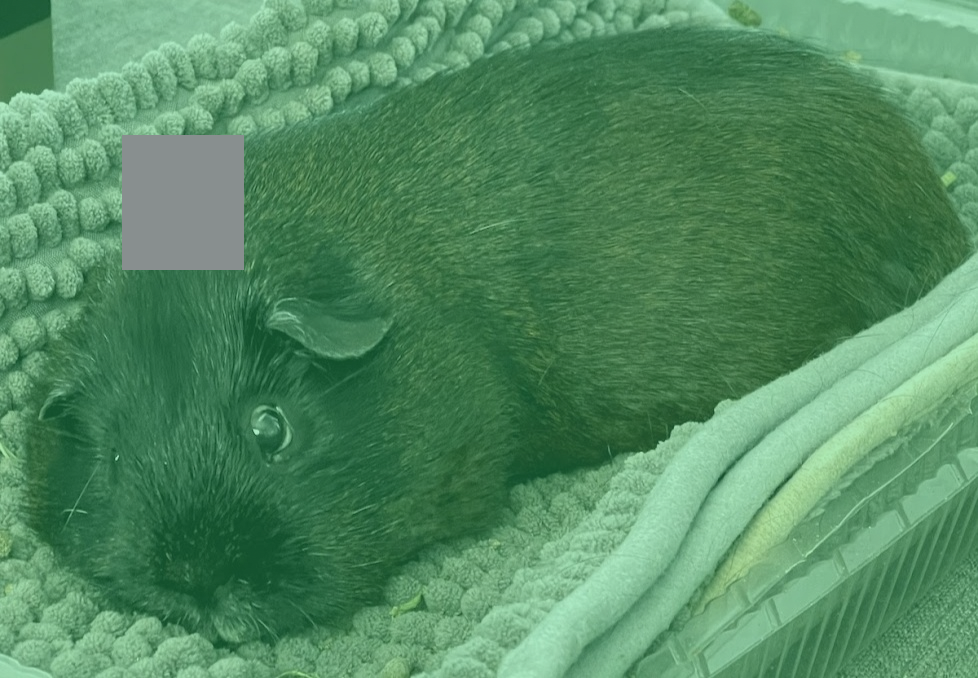
\includegraphics[width=\linewidth]{figures/fig_tampered_overlay.png}\\
    \footnotesize (a) Verification overlay
  \end{minipage}\hfill
  \begin{minipage}[t]{0.30\columnwidth}
    \centering
    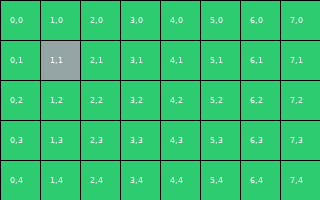
\includegraphics[width=\linewidth]{figures/fig_tampered_tilemap.png}\\
    \footnotesize (b) Tile map
  \end{minipage}
  \caption{Example verification output after localized tampering. GREEN
    tiles remain internally consistent, while RED tiles identify the
    tampered spatial region; the compact tile map is the machine-readable
    verification summary used for tile-level scoring.}
  \label{fig:tampered}
\end{figure}

\begin{table}[t]
  \centering
  \caption{Tile-level tamper detection by content class ($k{=}1$).}
  \label{tab:detection}
  \begin{tabular}{lccc}
    \toprule
    Content class & Images & Detection & FP rate \\
    \midrule
    Real photographs        & 94 & 100\% & 0\% \\
    Synthetic portrait      &  1 & 100\% & 0\% \\
    Synthetic landscape     &  1 & 100\% & 0\% \\
    Synthetic document      &  1 & 100\% & 0\% \\
    Synthetic geometric     &  1 & 100\% & 0\% \\
    Synthetic noise         &  1 & 100\% & 0\% \\
    \midrule
    \textbf{Total}          & \textbf{99} & \textbf{100\%} & \textbf{0\%} \\
    \bottomrule
  \end{tabular}
\end{table}

\subsection{Append Mode Performance}

Table~\ref{tab:append} reports wall-clock speedup of append mode versus
full re-encode for the implementation benchmark. The benchmark varies
the preserved prefix of each affected tile chain, not the fraction of
tiles modified. The largest measured gain ($74.2\%$ faster) occurs when
the final quarter of blocks is rewritten in a $2048{\times}2048$ image;
the smallest measured gain ($13.5\%$ faster) occurs when the final
three quarters of blocks are rewritten in a $512{\times}512$ image.

\begin{table}[t]
  \centering
  \caption{Append mode speedup vs.\ full re-encode.}
  \label{tab:append}
  \begin{tabular}{lcc}
    \toprule
    Scenario & Blocks rewritten & Speedup \\
    \midrule
    Best measured append case & ${\sim}25\%$ & $+74.2\%$ \\
    Worst measured append case & ${\sim}75\%$ & $+13.5\%$ \\
    Full re-encode & $100\%$     & baseline \\
    \bottomrule
  \end{tabular}
\end{table}

\subsection{Format Robustness}

Table~\ref{tab:format} reports PBC verification outcomes after
re-saving the embedded image in five lossless and five lossy formats.
Lossless formats preserve LSB data exactly; lossy formats corrupt it.
This defines the current deployment boundary: PBC is reliable in
lossless pipelines (PNG, TIFF, lossless WebP, BMP, raw TIFF)
and fails gracefully (GRAY verdict) in lossy ones. Consistent with the scope stated in Sections~\ref{sec:intro} and~\ref{sec:threat}, this is the intended operating regime, controlled editorial, archival, and wire-handoff workflows, and not arbitrary lossy social-media or messaging redistribution.

\begin{table}[t]
  \centering
  \caption{PBC verification after format re-save ($k{=}1$). Lossless
    formats preserve the embedded chain; lossy formats corrupt it.}
  \label{tab:format}
  \begin{tabular}{llc}
    \toprule
    Format           & Type     & Verification \\
    \midrule
    PNG              & Lossless & \textbf{PASS} \\
    TIFF             & Lossless & \textbf{PASS} \\
    Lossless WebP    & Lossless & \textbf{PASS} \\
    BMP              & Lossless & \textbf{PASS} \\
    Raw TIFF         & Lossless & \textbf{PASS} \\
    \midrule
    JPEG Q100        & Lossy    & FAIL (GRAY)  \\
    JPEG Q95         & Lossy    & FAIL (GRAY)  \\
    JPEG Q75         & Lossy    & FAIL (GRAY)  \\
    WebP Q90         & Lossy    & FAIL (GRAY)  \\
    WebP Q75         & Lossy    & FAIL (GRAY)  \\
    \bottomrule
  \end{tabular}
\end{table}

\subsection{PBC-Forest: Crop Survival}

Table~\ref{tab:forest} compares genesis-block survival between grid
mode and PBC-Forest after non-aligned crops removing $60$--$80\%$ of
the image area. In grid mode, a single-pixel misalignment between the
crop boundary and the tile grid destroys all block synchronization,
yielding zero recoverable genesis blocks regardless of how much of the
image survives. PBC-Forest's pseudo-random anchor placement ensures
that a statistically reliable fraction of anchors fall inside the
surviving region for any crop position or aspect ratio. We stress that this crop resilience addresses spatial excision specifically and should not be read as general robustness to lossy web or social-media transformations.

\begin{figure}[t]
  \centering
  \begin{minipage}[t]{0.32\columnwidth}
    \centering
    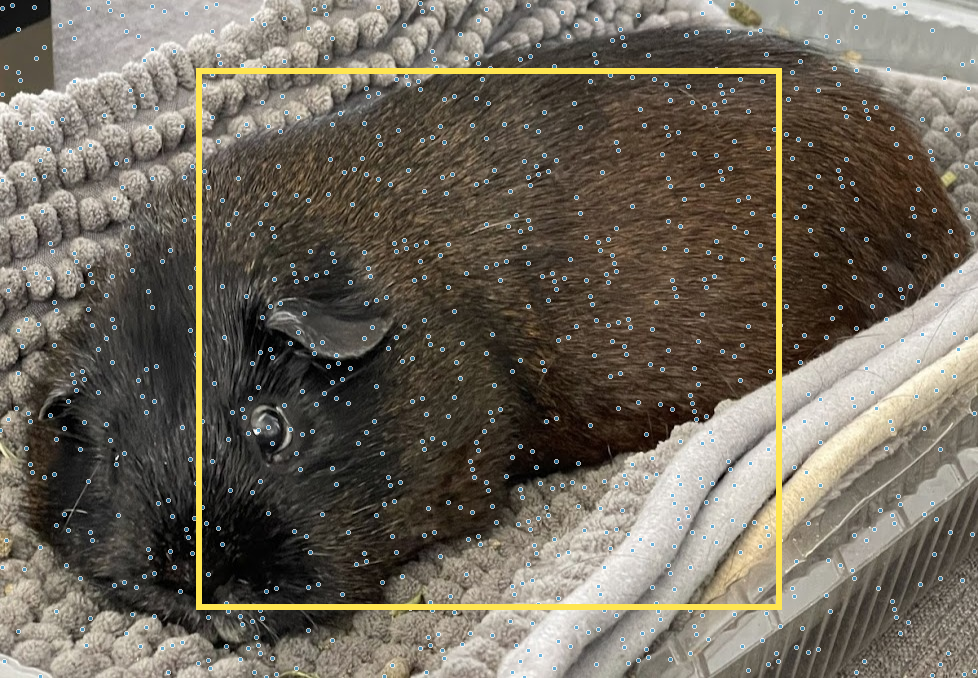
\includegraphics[width=\linewidth]{figures/fig_forest_before_crop.png}\\
    \footnotesize (a) Before crop
  \end{minipage}\hfill
  \begin{minipage}[t]{0.32\columnwidth}
    \centering
    
\includegraphics[width=\linewidth]{figures/fig_forest_after_crop.png}\\
    \footnotesize (b) After crop
  \end{minipage}\hfill
  \begin{minipage}[t]{0.32\columnwidth}
    \centering
    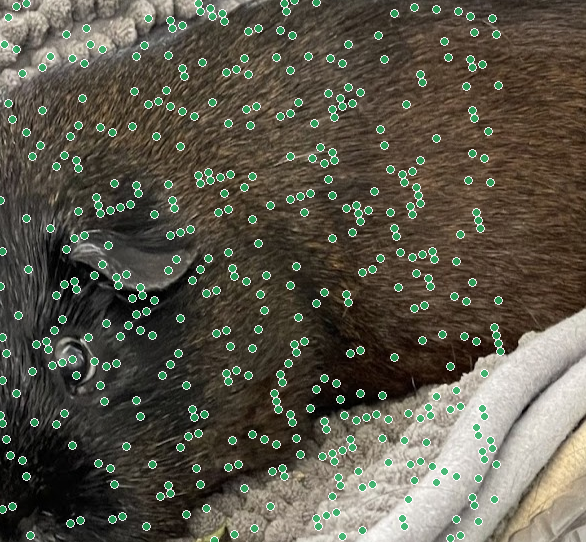
\includegraphics[width=\linewidth]{figures/fig_forest_survivors.png}\\
    \footnotesize (c) Genesis survivors
  \end{minipage}
  \caption{PBC-Forest verification example. Independently placed genesis
    anchors are scattered before redistribution, a non-aligned crop removes
    most spatial context, and the verifier still recovers the surviving
    anchors independently. In this fresh public-code run, the crop recovers
    $442/1000$ anchors ($44.2\%$), consistent with
    Table~\ref{tab:forest}.}
  \label{fig:forest_example}
\end{figure}

\begin{table}[!htbp]
  \centering
  \caption{Genesis block survival after non-aligned crop.}
  \label{tab:forest}
  \begin{tabular}{lcc}
    \toprule
    Mode            & Crop severity        & Survival \\
    \midrule
    Grid (baseline) & 60--80\%, non-aligned & 0\%         \\
    PBC-Forest      & 60--80\%, non-aligned & 41.1--44.6\% \\
    \bottomrule
  \end{tabular}
\end{table}

\subsection{Positioning vs.\ Neural Watermarking}

PBC and neural watermarking schemes such as
EditGuard~\cite{editguard} and OmniGuard~\cite{omniguard} occupy
complementary regimes. PBC is fragile and learning-free, with
tile-level granularity and zero-GPU deployment; neural methods are
robust to lossy channels with pixel-level granularity, at the cost of
training data and GPU inference. We do not benchmark on shared test
images because the design points differ at the channel-robustness
axis: PBC targets lossless distribution paths, where neural robustness
offers no advantage; neural methods target the lossy-survival regime
PBC explicitly does not address. We therefore present this comparison as a positioning statement rather than a claim of superiority.

\subsection{Limitations}
\label{sec:limitations}

\emph{Evaluation scope.} The current benchmark uses 99 images with
synthetic rectangular tampering. Evaluation against realistic forensic
manipulation scenarios such as copy-move, splicing, and neural
inpainting, and on larger and more diverse image corpora, is needed to
characterize detection boundaries more precisely.

\emph{Content-aware tamper.} Our tamper experiments overwrite affected
regions with random pixel values, destroying LSBs by construction.
Modifications that preserve LSB structure (e.g., careful inpainting
onto the original LSBs) are not yet evaluated in this paper.

\emph{Identity binding.} The originator ID is self-asserted.
Cryptographic binding (e.g., Ed25519 signature over each block) is a
planned extension; as stated in the threat model, PBC does not by itself authenticate the originator or provide signed provenance.

\emph{Lossy channels.} PBC yields a GRAY verdict after lossy
re-encoding and is reliable only on lossless distribution paths.

\emph{Scale and sensitivity.} Behavior on very high-resolution imagery
($\gg$4\,MP), and sensitivity sweeps over Forest anchor count $N_f$
and append-fraction crossover, are characterized in the public
reference implementation but not reported here.

\emph{Structural manipulation.} Cascade isolation
(Lemma~\ref{lem:isolation}) guarantees that each tile is verified
independently, but this independence also means that the system
cannot detect cross-tile manipulations such as tile swapping or
clone displacement. Two visually similar tiles (e.g., sky or grass
regions) can be exchanged without breaking either tile's internal
chain. This is a direct consequence of the absence of global
geometric awareness across tiles.

% ============================================================
\section{Conclusion}
\label{sec:conclusion}

This paper presented Pixel Block Chain (PBC), a lightweight,
learning-free watermarking scheme for spatial tamper localization and
redistribution-resilient Edit Ledger recovery. The grid-of-chains architecture
provides a formally proved cascade-isolation property that is absent
from prior single-chain schemes, ensuring that integrity failure in one
region does not propagate to adjacent tiles. The per-tile Edit Ledger
enables append-mode partial rewriting with up to 74.2\% speedup in the
measured append-depth benchmark, supporting practical editorial
workflows where only a subset of the image is modified.

PBC-Forest extends this foundation to crop-heavy distribution paths,
delivering 41.1 to 44.6\% genesis-block survival after severe
non-aligned cropping where the regular-grid baseline offers no
recovery. This result is directly relevant to the crop-and-reshare
workflows that dominate social-media distribution.

The current deployment target is controlled, lossless channels. Four
directions for future work follow naturally from the limitations
identified above. First, JPEG robustness via DCT-domain embedding, placing watermark symbols
in mid-frequency coefficients that survive quantization, trading PSNR for survival, would extend
PBC to lossy distribution paths. Second, embedding absolute tile coordinates and a cross-tile commitment (e.g., a Merkle root over all tile genesis hashes) into
each append block would enable detection of structural manipulations
such as tile swapping or clone displacement, addressing the geometric
blindness inherent in the current isolation property. Third, formal trust-model integration with manifest-based provenance standards such as C2PA, clarifying which properties, tile-local integrity and edit continuity, PBC provides on its own and which, originator authentication and container-level provenance, require external signed infrastructure, together with adversarial analysis of the guarantees a pixel-embedded Edit Ledger can and cannot offer independently. Fourth, evaluation on
larger and more forensically representative benchmarks, including
realistic manipulation scenarios, is needed to characterize detection
boundaries beyond the synthetic tampering model used here. The
reference implementation is publicly
available.\footnote{\url{https://github.com/flegare/pixel-block-chain}}


\section*{Acknowledgments}

Generative AI tools were used under author supervision: Claude Opus 4 (Anthropic), accessed via GitHub Copilot, assisted with reference-implementation development, and Paperpal AI assisted with language refinement. All AI-assisted code and text were reviewed, verified, and edited by the authors, who take full responsibility for the content.

% ============================================================
\bibliographystyle{IEEEtran}

\begin{thebibliography}{15}

\bibitem{c2pa_spec}
  C2PA, ``Content Credentials: C2PA Technical Specification v2.4,''
  Coalition for Content Provenance and Authenticity, Apr. 2026. [Online].
  Available: \url{https://spec.c2pa.org/specifications/specifications/2.4/}

\bibitem{he2008blockchain}
  Z.~He, W.~Zhang, and H.-T.~Tai,
  ``Block-Chain Based Fragile Watermarking Scheme with Superior
  Localization,''
  in \emph{Proc. 10th Int'l Workshop on Information Hiding},
  LNCS vol.~5284, pp.~147--160, Springer, 2008.

\bibitem{fang2020blockchain}
  W.~Fang, Y.~Wang, and X.~Wang,
  ``Image Tampering Location and Restoration Watermarking Based on
  Blockchain Technology,''
  in \emph{Big Data Analytics for Cyber-Physical System in Smart City},
  vol.~1117, Springer, 2020.

\bibitem{editguard}
  Z.~Zhang, M.~Wu, Y.~Zheng, and X.~Sun,
  ``EditGuard: Versatile Image Watermarking for Tamper Localization
  and Copyright Protection,''
  in \emph{Proc. IEEE/CVF CVPR}, pp.~11--20, 2024.

\bibitem{omniguard}
  X.~Zhang, Z.~Tang, Z.~Xu, R.~Li, Y.~Xu, B.~Chen, F.~Gao,
  and J.~Zhang,
  ``OmniGuard: Hybrid Manipulation Localization via Augmented Versatile
  Deep Image Watermarking,''
  in \emph{Proc. IEEE/CVF Conference on Computer Vision and Pattern
  Recognition (CVPR)}, pp.~3008--3018, 2025.

\bibitem{cox2007watermarking}
  I.~Cox, M.~Miller, J.~Bloom, J.~Fridrich, and T.~Kalker,
  \emph{Digital Watermarking and Steganography}, 2nd~ed.
  Morgan Kaufmann, 2007.

\bibitem{korus2017survey}
  P.~Korus,
  ``Digital image integrity---a survey of protection and verification
  techniques,''
  \emph{Digital Signal Processing}, vol.~71, pp.~1--26, 2017.

\bibitem{lin2001semifragile}
  C.-Y.~Lin and S.-F.~Chang,
  ``A Robust Image Authentication Method Distinguishing JPEG Compression
  from Malicious Manipulation,''
  \emph{IEEE Trans. Circuits Syst. Video Technol.},
  vol.~11, no.~2, pp.~153--168, Feb.~2001.

\bibitem{aythora2020origin}
  J.~Aythora et~al.,
  ``Multi-Stakeholder Media Provenance Management to Counter Synthetic
  Media Risks in News Publishing,''
  in \emph{Proc. Int'l Broadcasting Convention (IBC)}, 2020.

\bibitem{corvi2023synthetic}
  R.~Corvi, D.~Cozzolino, G.~Zingarini, G.~Poggi, K.~Nagano,
  and L.~Verdoliva,
  ``On the Detection of Synthetic Images Generated by Diffusion
  Models,''
  in \emph{Proc. IEEE Int'l Conf. Acoustics, Speech and Signal
  Processing (ICASSP)}, pp.~1--5, 2023.

\bibitem{coco_dataset}
  T.-Y.~Lin et~al.,
  ``Microsoft COCO: Common Objects in Context,''
  in \emph{Proc. European Conference on Computer Vision (ECCV)},
  pp.~740--755, 2014.

\bibitem{flowers_dataset}
  M.-E.~Nilsback and A.~Zisserman,
  ``Automated Flower Classification over a Large Number of Classes,''
  in \emph{Proc. Indian Conference on Computer Vision, Graphics and
  Image Processing}, 2008.

\bibitem{pets_dataset}
  O.~M.~Parkhi, A.~Vedaldi, A.~Zisserman, and C.~V.~Jawahar,
  ``Cats and Dogs,''
  in \emph{Proc. IEEE CVPR}, 2012.

\bibitem{sherman2021indicators}
  I.~N.~Sherman, J.~W.~Stokes, and E.~M.~Redmiles,
  ``Designing Media Provenance Indicators to Combat Fake Media,''
  in \emph{Proc. 24th Int'l Symp. on Research in Attacks, Intrusions
  and Defenses (RAID)}, pp.~324--339, 2021.

\bibitem{feng2023provenance}
  K.~J.~K.~Feng, N.~Ritchie, P.~Blumenthal, A.~Parsons,
  and A.~X.~Zhang,
  ``Examining the Impact of Provenance-Enabled Media on Trust and
  Accuracy Perceptions,''
  \emph{Proc. ACM Human-Computer Interaction},
  vol.~7, no.~CSCW2, pp.~1--42, 2023.

\end{thebibliography}
\end{document}
